\documentclass[titlepage,a4paper]{jsarticle}
\usepackage{../../sty/import}%各種パッケージインポート
\usepackage{../../sty/title_team}%タイトルページの変更
% レポートタイトル
\title{球体-木製ブロック衝突実験の\\重回帰分析を用いた分析}
% 提出日
\expdate{\today}
% 科目名
\subject{情報システム工学実験}
% 分野
\class{情報経営システム工学分野}
% 学年
\grade{B3}
% 学籍番号
\mynumber{学籍番号}
% 記述者
\author{本間三暉}
% グループ名
\team{10}
\begin{document}
\maketitle
\section{はじめに}
% 本実験の目的や行ったことを記述
\subsection{前置き}
今回の実験で物理実験を行うに当たり,16班に分かれ,各班ごとに実験を行い実験結果をExcelにまとめた.
その実験結果を一つにまとめる際ラベル等の指定がなかったため,おおよそデータの分析を行うとは思えないような形式でまとめている班が散見された.

そのため,各班に呼びかけ形式の統一を行うよう呼びかけた.
しかし,レポート執筆時点(2024年6月27日)で,形式の統一が行われておらずどの数字が実験データかわからない班が3班,単位が正しく直されていなさそうな班が1班いた.

そのような数字はデータの前処理の段階で排除したため,16班分のデータを用いた想定通りのデータ分析が行えないことを断っておきたい.
また,形式を統一した際に,平均値のみを提出した班と生データを提出した班があるため,データの数に偏りがあることも断っておきたい.

\subsection{目的}
現代社会において,データサイエンスの重要性はますます高まっている.
データサイエンスとは,与えられたデータに基づいて知見を見出し,その知見を次の行動に活かすことを目的としている.
本レポートでは,データ分析の基本的な手法とその応用について実験を通じて探求する.

本実験は,データ分析の5つの手順(PPDACサイクル)に基づいて進められる.
PPDACサイクルは,問題の把握(Problem),調査の計画(Plan),データの収集(Data),データの分析(Analysis),および結論の考(Conclusion)
の5つのステップから成り立つ.
これらのステップを踏むことで,データから有用な情報を引き出し,具体的な課題解決に繋げることを目指す.

本レポートの目的は,実験を通じてデータ分析の基本的な手法を理解し,実際のデータを用いた分析のプロセスを経験することである.
さらに,得られた知見をもとに具体的な解決策を提案し,実務に応用できるスキルを身につけることを目指す.

\section{データ(実験概要)}
% どのような実験装置でどういったデータを取ったかを記述
% 他の球体とブロックを使った実験データは,他のグループのデータを採用する.
今回の実験では,図\ref{実験装置}のような装置を用いて行う.
\begin{figure}[H]
  \centering
  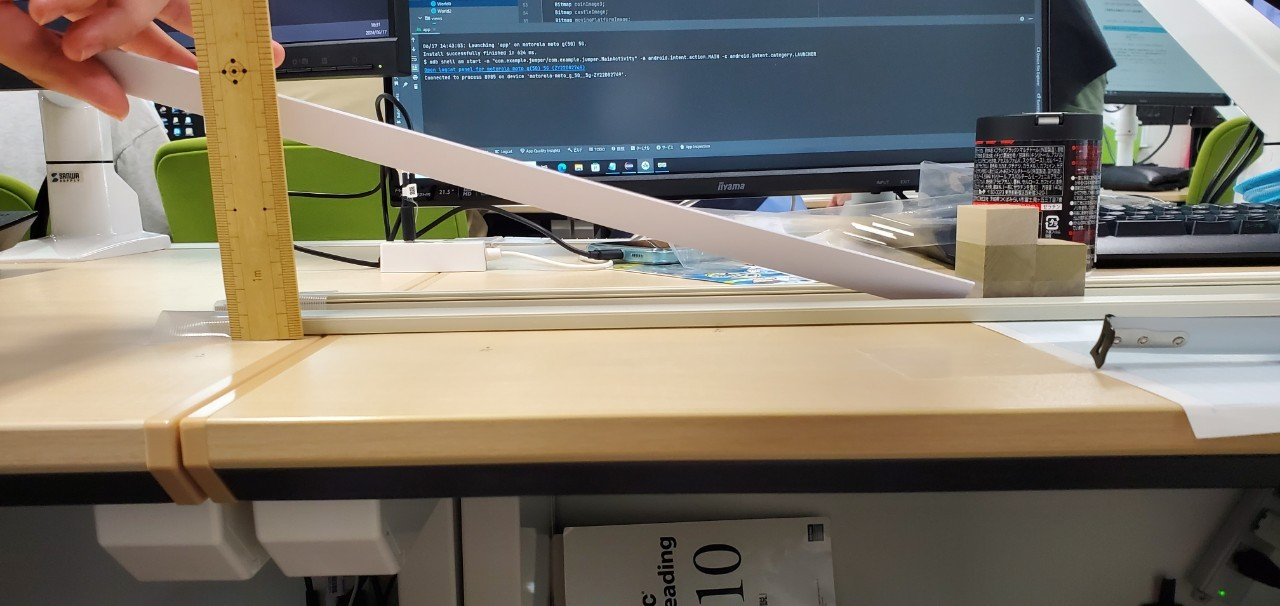
\includegraphics[width=12cm]{img/data_science1.jpg}
  \caption{実験装置}
  \label{実験装置}
\end{figure}

今回,私の班はボールが転がり始める高さ(以下高さ),ボールが転がった距離の内地面と平行な向きに移動した距離(以下底辺),物体の移動距離(以下移動距離)を測定し,
ボールが転がる距離(以下斜辺),斜辺と底辺のなす角(角度)などは計算で導出することにした.
斜辺の導出方法は,斜辺を$C$,高さを$A$,底辺を$B$とした時,三平方の定理から式\eqref{Pythagoras}で導出できる.
\begin{align}
  C^{2} & = A^{2} + B^{2}                           \\
  C     & = \sqrt{A^{2} + B^{2}} \label{Pythagoras}
\end{align}

また,角度は測定値である高さと底辺から導出する.
高さを$A$,底辺を$B$,角度を$\theta$とした時,タンジェントの定義式から,アークタンジェントを用いた式\eqref{atan}から導出できる.
\begin{align}
  \tan \theta & = \frac{A}{B}                                   \\
  \theta      & = \arctan \left(\frac{A}{B}\right) \label{atan}
\end{align}

Excelの関数ATAN()は戻り値の単位がラジアンなので,これを度数法に直す必要がある.
弧度法は,扇形を考えた時,中心角$\theta$は円弧の長さ$l$に比例する.
円弧の長さ$l$と扇型の半径$r$の比をとると,同じ角度$\theta$に対して扇型の大きさにかかわらずこの比は一定である.
このような性質を利用して,角度の大きさは式\eqref{rad}を用いて定義されている.
\begin{align}
  \theta & = \frac{l}{r}\label{rad}
\end{align}

よって弧度法から度数法に変換するためには,弧度法の角度を$\theta$,度数法の角度を$\theta'$とした時,式\eqref{convert}を用いれば良い.
\begin{align}
  \theta' & = \frac{360}{2\pi}\theta \label{convert}
\end{align}

また,今回は情報経営システム工学分野B3の学生を4人で1つの班に分け,全部で16班作成する.
各班ごとに使用するボールの重さや材質,物体の重さを変え実験を行う.
ボールの種類は以下の7種類である.
\begin{itemize}
  \item 鉄球1
  \item 鉄球2
  \item 鉄球3
  \item ビー玉1
  \item ビー玉2
  \item スーパーボール
  \item ゴムボール
\end{itemize}
また,物体の重さは5段階である.

私の班は重さが$66.9[g]$の鉄球をボールに用いて,重さが$25.7[g]$で地面との接地面積が$1350[mm^{2}]$の物体を用いて実験を行った.


\section{データの前処理}
% 前処理で行ったことを記述
\subsection{データの前処理について}
データの前処理は,データ分析工程の8割を占めるとも言われるほど重要な工程である.
必要な情報が完璧にそろっているデータは珍しく,多くのデータは必要な数値が抜けている場合がほとんどである.
さらに,データごとに形式が違うこともあり,数値に変換されていないテキストデータ(文字データ)しかない場合も多々ある.
このような状態のデータではエラーが発生しやすく,不十分な結果しか得られないため,データの前処理を行って事前にデータを整理する必要がある.
データの形式や質・量が予測精度を決定するため,前処理はスムーズに分析を行うために不可欠であり,予測精度を担保するための重要な開発工程である.

データの前処理には大きく分けて5つの方法がある.
\subsubsection{数値型への変換}
本来数値型が入力されるべき場所に文字列や記号が入力されている場合がある.
例えば,Excelのデータで他の欄には数値データが入っているにもかかわらず,一箇所に「測定不可」のようなメモが残されている場合がある.
そのような文字列データを除去し,全てのデータを数値型に置き換える必要がある.

\subsubsection{欠損値処理}
欠損値とは,何らかの理由により記載されなかったり欠落したりした値のことである.欠損値の対処法としては以下の方法がある.
\begin{itemize}
  \item 平均値や最頻値で補完する:欠損値を含むデータが分析に必要な場合は,平均値や最頻値で補完する.
        欠損値を含むデータを全て除外するとデータ数が不足する場合などは,できる限り補完を検討する.
  \item 行または列ごと除外する:欠損値の割合が高い行や列がある場合は,そのデータを分析対象から除外する.
\end{itemize}
\subsubsection{外れ値処理}
ヒストグラムや散布図を用いてデータの分布を確認し,外れ値の有無を確認する.外れ値の対処法としては以下のようなものがある.
\begin{itemize}
  \item 正しい値に修正する:外れ値がデータの入力ミスやシステムのエラーによる場合は,正しい値に修正する.
  \item 行ごと除外する:外れ値が分析結果に大きな影響を与える場合は,行ごと除外する.
  \item そのまま使用する:外れ値が分析結果に影響しない場合は,そのまま使用することもある.
\end{itemize}
\subsubsection{スケーリング}
データの値を特定の範囲に変換する前処理方法である.
例えば,異なる単位のデータを比較する際に単位をそろえたり,データの値を同じスケールにそろえたりするためによく使われるスケーリングの手法には,
「Min-Maxスケーリング」や「Zスコアスケーリング」などがある.
\begin{itemize}
  \item Min-Maxスケーリングはデータを最小値0,最大値1にスケーリングする方法である.
  \item Zスコアスケーリングは平均0,分散1にスケーリングする方法で,大きな外れ値がある場合に適している.
  \item Robustスケーリングは,データの中央値を0,四分位範囲を1として変換する手法で,外れ値の影響を受けにくい.
\end{itemize}
\subsubsection{ダミーデータ}
ダミー変数の作成がある.質的データやカテゴリカルデータを数字に変換する手法であり,例えばカテゴリを「0」と「1」に変換する方法がある.
例えば,「はい」を1,「いいえ」を0にしたり,「男」を1,「女」を0に変換する.
3つ以上のカテゴリがある場合は,各カテゴリを1とし,その他を0とした数列に変換する.
\subsection{グループデータ}
% ・グループデータ
実験時にデータを取得した際,高さ$200[mm]$,底辺$100[mm]$のときボールが物体を弾いてしまい上手くデータが取れなかったため,"N/A"と記述した.
しかし,データ分析の際にはそのようなデータは不要なため行ごと削除した.
\subsection{統合データ}
% ・全グループ統合データ
実験時各班でデータを作成したため,フォーマットや基準にする単位がバラバラになってしまっていた.
それだけならいいが,表を横に作成する班,シートを増やしすぎている上に名前を変えずそもそもデータがどこにあるか分かりにくい班,
単位を明記していない班など様々であった.

そのため,各班ごとにフォーマットとデータの単位を表\ref{テンプレ}のような形に整形するよう呼びかけた.また,表が横に長いため途中で折り返して示す.
\begin{table}[H]
  \centering
  \caption{整形後フォーマット}
  \label{テンプレ}
  \begin{tabular}{lllll}
    移動距離{[}mm{]}    & 底辺{[}mm{]}                       & 高さ{[}mm{]}                       & 斜辺{[}mm{]} & 理論値角度{[}度{]}                      \\\hline\hline
    20              & 430                              & 100                              & 441.475    & 13.092                            \\\hline
    理論値角度{[}ラジアン{]} & \multicolumn{1}{r}{球体の質量{[}g{]}} & \multicolumn{1}{r}{物体の質量{[}g{]}} & 球体の種類      & 物体の底面積{[}mm\textasciicircum{}2{]} \\\hline\hline
    0.228           & 5.5                              & 10.5                             & 鉄球1        & 1305                              \\\hline
  \end{tabular}
\end{table}

呼びかけの結果,多くの班でデータのフォーマットが統一された.
フォーマットを統一してくれず基準にした単位も記述されていないような修正のしようがない班のデータは除外した.
また,ボールの素材によって別の分析をする必要があったのでダミー変数を追加した.
ダミー変数を追加する際,式\eqref{excel}に示すExcel関数を用いて作成した.
\begin{align}
  =IF(MID(\$I2,1,1)="鉄",1,0) \label{excel}
\end{align}

ここで,セル$I2$は球体の種類の列の値である.
この式は球体の種類の列を参照し,1文字目が"鉄"であったら1,そうでなかったら0を入力する関数である.
各グループの実験で用いたボールがどの素材であるかは1文字目を参照し,ダミー変数を1にしたい材質の1文字目と比べれば良い.

このようにして表\ref{テンプレ}の右に追加したダミー変数を表\ref{ダミー}に示す.
\begin{table}[H]
  \centering
  \caption{ダミー変数追加}
  \label{ダミー}
  \begin{tabular}{llll}
    鉄球 & ビー玉 & ゴムボール & スーパーボール \\\hline\hline
    1  & 0   & 0     & 0       \\\hline
  \end{tabular}
\end{table}

このように処理したデータを用いて分析を行う.


\section{相関分析・単回帰分析}\label{相関}
私のグループで取ったデータに関して相関分析と単回帰分析を行う.
\subsection{相関分析}
相関分析とは,2つの変数間の関係性を定量的に評価する統計手法である.
この分析手法は,様々な分野で広く活用されており,データに隠れた関係性を発見し,因果関係の手がかりを得るために重要な役割を果たしている.

相関分析では,2つの変数間の関係の強さと方向を相関係数によって表現する.
相関係数は-1から1の間の値を取り,1に近いほど正の相関が強く,-1に近いほど負の相関が強いことを示す.
0に近い値は,相関がほとんどない,または全くないことを意味する.

相関分析を行う際には,まず散布図を作成して変数間の関係を視覚的に確認することが重要である.
散布図から関係のパターン(線形,非線形など)を把握した上で,相関係数を計算し,その値に基づいて相関の強さを解釈する.

ただし,相関分析の結果を解釈する際には,いくつかの注意点がある.
相関があることは因果関係を意味するわけではなく,第三の要因が両方の変数に影響を与えている可能性もある.
また,相関係数は外れ値に敏感であるため,データの前処理で外れ値の処理が重要となる.
さらに,Pearsonの相関係数は線形関係を前提としているため,非線形の関係がある場合には他の方法を検討する必要がある.

具体的なデータセットに対して相関分析を適用する際は,データの特性に応じた前処理が必要となる.
例えば,カテゴリカルデータを数値に変換するためにダミー変数を使用したり,変数のスケールを揃えるために標準化を行ったりする.
このように,相関分析は変数間の関係性を理解するための強力なツールであり,適切に使用することで,データから有益な知見を得ることができる.
しかし,分析結果の解釈には注意が必要であり,常に因果関係の可能性を念頭に置きながら,多角的な視点でデータを見ることが重要である.

この実験ではExcelの機能を用いて相関分析を行う.
相関分析を行った結果について\ref{相関分析}に示す.
\begin{table}[H]
  \caption{相関分析}
  \label{相関分析}
  \begin{tabular}{c|lllll}
                 & 移動距離{[}mm{]} & 底辺{[}mm{]}  & 高さ{[}mm{]}  & 斜辺{[}mm{]}   & 理論値角度{[}度{]} \\\hline\hline
    移動距離{[}mm{]} & 1            &             &             &              &              \\
    底辺{[}mm{]}   & 0.456861417  & 1           &             &              &              \\
    高さ{[}mm{]}   & 0.898531378  & 0.136363636 & 1           &              &              \\
    斜辺{[}mm{]}   & 0.616331666  & 0.972160283 & 0.352605016 & 1            &              \\
    理論値角度{[}度{]} & 0.25097754   & -0.66280947 & 0.589354047 & -0.476740815 & 1            \\\hline
  \end{tabular}
\end{table}
これを見ると,移動距離と高さの正の相関が強いことがわかる.
\subsection{単回帰分析}

\section{重回帰分析}
\subsection{グループデータ}
% ・球体・ブロック各1種のグループデータで行った重回帰分析について記述
%  説明変数の選択方法
%  重回帰式
%  修正済決定係数とあてはまりのよさを記述
% P 値と説明力について記述
% ※余裕があれば未計測の説明変数値での計算予測値と実測値の比較をしてみる

\subsection{全グループデータ}
% ・全グループデータを合わせた重回帰分析について記述
%  説明変数の選択方法
%  重回帰式
%  修正済決定係数とあてはまりのよさを記述
% P 値と説明力について記述
% ※余裕があれば未計測の組み合わせ等での計算予測値と実測値の比較をしてみる

\section{おわりに}
\subsection{結論}
% 本分析の結論として考えられる特徴を記述
\subsection{考察}
% 木製ブロックの移動距離に影響する要素は~等
\subsection{反省点}
% 反省点:球体の種類のデータ数に偏りがあった.全種類バランスよくデータを取れるように実験計画を見直す必要がある.

\subsection{要望}
% テンプレートの統一等について,来年以降の学生に向けて欠点をお願いすること
\begin{itemize}
  \item \ref{相関}節の解説がなかったので,"スライドを参照すること"などでいいので多少書いてもらえると嬉しかった.
  \item データを入力する時に班によってフォーマットや基準にする単位が違い,
        全グループの統合データを作成するのがとても大変だったので,
        先生の方から表\ref{テンプレ}に示すようなテンプレートファイルを配布し,フォーマットや単位の統一を促してほしかった.
  \item iliasにレポートの提出場所を作るのが提出期限の直前になってしまっていたので実験が終わり次第すぐ上げてもらえると嬉しかった.
        また,そこにwordのテンプレートをつけてほしい.
  \item
\end{itemize}
\end{document}